% 图 6.20 布洛赫壁 (a) 与奈尔壁 (b) 三维示意：磁化分别在壁面内 / 膜面内旋转 180 度
\documentclass[tikz,border=5pt]{standalone}
\usetikzlibrary{arrows.meta}
\usepackage{amsmath}
\usepackage{bm}
\usepackage{fontspec}
\setmainfont{Times New Roman}
\begin{document}
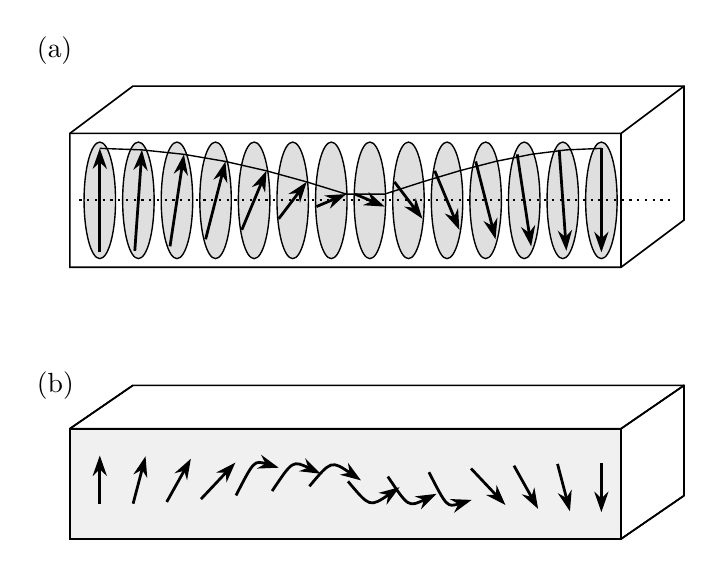
\begin{tikzpicture}[line width=0.8pt,>=Stealth]
\pgfmathsetmacro{\N}{13}
% ================= (a) Bloch wall =================
\node[anchor=west] at (-0.55,2.75) {(a)};
% box: front face (0,0)-(7,1.7), depth (0.8,0.6)
\draw[line width=0.6pt] (0,0) -- (7,0) -- (7.8,0.6) -- (7.8,2.3) -- (0.8,2.3) -- (0,1.7) -- cycle;
\draw[line width=0.6pt] (0,1.7) -- (7,1.7) -- (7.8,2.3);
\draw[line width=0.6pt] (7,0) -- (7,1.7);
% disk chain
\foreach \i in {0,...,13} {
  \pgfmathsetmacro{\xx}{0.38+\i*0.49}
  \pgfmathsetmacro{\ph}{90-\i*(180/13)}
  \pgfmathsetmacro{\dx}{0.19*cos(\ph)}
  \pgfmathsetmacro{\dy}{0.66*sin(\ph)}
  \fill[gray!25] (\xx,0.85) ellipse (0.20 and 0.74);
  \draw[line width=0.5pt] (\xx,0.85) ellipse (0.20 and 0.74);
  \draw[->,line width=1pt,>={Stealth[length=2.6mm,width=1.8mm]}] (\xx-\dx,0.85-\dy) -- (\xx+\dx,0.85+\dy);
}
% dotted wall-normal line through disk centres
\draw[dotted,line width=0.8pt] (0.12,0.85) -- (7.62,0.85);
% spiral trajectory of arrow tips
\def\tip{}
\foreach \i in {0,...,13} {
  \pgfmathsetmacro{\xx}{0.38+\i*0.49}
  \pgfmathsetmacro{\ph}{90-\i*(180/13)}
  \pgfmathsetmacro{\tx}{\xx+0.19*cos(\ph)}
  \pgfmathsetmacro{\ty}{0.85+0.66*abs(sin(\ph))}
  \ifnum\i=0 \xdef\tip{(\tx,\ty)}\else \xdef\tip{\tip -- (\tx,\ty)}\fi
}
\draw[line width=0.5pt] \tip;
% ================= (b) Neel wall =================
\node[anchor=west] at (-0.55,-1.5) {(b)};
\begin{scope}[shift={(0,-3.45)}]
  % box: front face (0,0)-(7,1.4), depth (0.8,0.55)
  \draw[line width=0.6pt] (0,0) -- (7,0) -- (7.8,0.55) -- (7.8,1.95) -- (0.8,1.95) -- (0,1.4) -- cycle;
  \draw[line width=0.6pt] (0,1.4) -- (7,1.4) -- (7.8,1.95);
  \draw[line width=0.6pt] (7,0) -- (7,1.4);
  \fill[gray!12] (0,0) rectangle (7,1.4);
  \draw[line width=0.6pt] (0,0) rectangle (7,1.4);
  \draw[line width=0.6pt] (0,1.4) -- (0.8,1.95);
  \draw[line width=0.6pt] (7,1.4) -- (7.8,1.95);
  \draw[line width=0.6pt] (7,0) -- (7.8,0.55);
  % rotating arrows in the film plane
  \foreach \i in {0,...,13} {
    \pgfmathsetmacro{\xx}{0.38+\i*0.49}
    \pgfmathsetmacro{\ph}{90-\i*(180/13)}
    \pgfmathsetmacro{\dx}{0.28*cos(\ph)}
    \pgfmathsetmacro{\dy}{0.26*sin(\ph)}
    \pgfmathsetmacro{\ex}{0.38*cos(\ph)}
    \pgfmathsetmacro{\ey}{0.36*sin(\ph)}
    \pgfmathsetmacro{\bu}{\ph>=0 ? 1 : -1}
    \ifdim\ph pt>-45pt \ifdim\ph pt<45pt
      \draw[->,line width=1pt,>={Stealth[length=2.6mm,width=1.8mm]}]
        (\xx-\dx,0.7-\dy) .. controls (\xx,0.7+\bu*0.3) .. (\xx+\ex,0.7+\ey);
    \else
      \draw[->,line width=1pt,>={Stealth[length=2.6mm,width=1.8mm]}]
        (\xx-\dx,0.7-\dy) -- (\xx+\ex,0.7+\ey);
    \fi\else
      \draw[->,line width=1pt,>={Stealth[length=2.6mm,width=1.8mm]}]
        (\xx-\dx,0.7-\dy) -- (\xx+\ex,0.7+\ey);
    \fi
  }
\end{scope}
\end{tikzpicture}
\end{document}
